\subsection{Breites}

\begin{frame}[fragile]{\texttt{\textbackslash OverfullCenter}}
  \begin{lstlisting}
  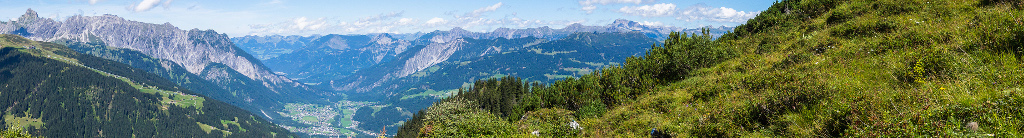
\includegraphics[width=\textwidth+25pt]{figures/Panorama.jpg}
  \end{lstlisting}

  \vspace{5pt}
  \rlap{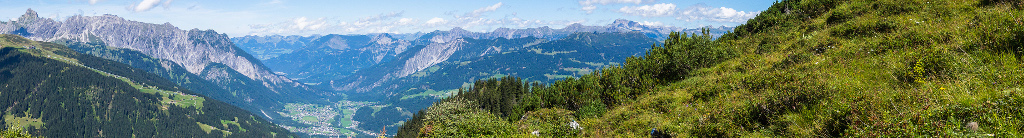
\includegraphics[width=\textwidth+25pt]{figures/Panorama.jpg}}

  \vspace{5pt}
  Bild oder Tabelle ist zu Breit, passt aber auf die Seite.\\
  Wie kriegt man es in die Mitte?

  \vspace{5pt}
  \begin{lstlisting}
  \OverfullCenter{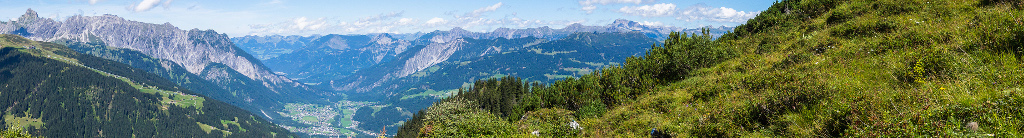
\includegraphics[width=\textwidth+25pt]{figures/Panorama.jpg}}
  \end{lstlisting}

  \vspace{5pt}
  \OverfullCenter{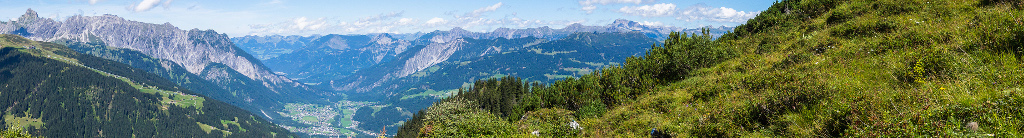
\includegraphics[width=\textwidth+25pt]{figures/Panorama.jpg}}

  \begin{block}{Code}
    \begin{lstlisting}
      \newcommand\OverfullCenter[1]{\noindent\makebox[\linewidth]{#1}}
    \end{lstlisting}
  \end{block}
\end{frame}

\begin{frame}[fragile]{\texttt{pdflscape}}
  Falls das Bild oder die Tabelle wirklich breiter als die Seite ist, ist vielleicht eine gedrehte Seite die Lösung.
  \begin{columns}[onlytextwidth, t]
    \begin{column}{0.50\textwidth}
      \begin{Packages}
        \begin{lstlisting}
          \usepackage{pdflscape}
        \end{lstlisting}
      \end{Packages}
      \begin{block}{Code}
        \begin{lstlisting}
          \begin{landscape}
            \begin{table}
              % .
            \end{table}
          \end{landscape}
        \end{lstlisting}
      \end{block}
    \end{column}
    \begin{column}{0.46\textwidth}
      \begin{itemize}
        \item Inhalt der \texttt{landscape}-Umgebung wird horizontal gesetzt (separate Seite)
        \item Seite wird im PDF-Reader horizontal angezeigt → schöner zu lesen
      \end{itemize}
    \end{column}
  \end{columns}
\end{frame}

\begin{landscape}
  \begin{frame}
    \centering
    $\langle$insert wide table here$\rangle$
  \end{frame}
\end{landscape}
